% Copyright 2004 by Till Tantau <tantau@users.sourceforge.net>.
% * <ferranpujolcamins@gmail.com> 2016-12-11T20:45:40.856Z:
%
% ^.
%
% In principle, this file can be redistributed and/or modified under
% the terms of the GNU Public License, version 2.
%
% However, this file is supposed to be a template to be modified
% for your own needs. For this reason, if you use this file as a
% template and not specifically distribute it as part of a another
% package/program, I grant the extra permission to freely copy and
% modify this file as you see fit and even to delete this copyright
% notice. 

\documentclass{beamer}
\usepackage[utf8]{inputenc}
\usepackage[T1]{fontenc}

\usepackage{color}
\usepackage{listings}


% There are many different themes available for Beamer. A comprehensive
% list with examples is given here:
% http://deic.uab.es/~iblanes/beamer_gallery/index_by_theme.html
% You can uncomment the themes below if you would like to use a different
% one:
%\usetheme{AnnArbor}
%\usetheme{Antibes}
%\usetheme{Bergen}
%\usetheme{Berkeley}
%\usetheme{Berlin}
%\usetheme{Boadilla}
%\usetheme{boxes}
%\usetheme{CambridgeUS}
%\usetheme{Copenhagen}
%\usetheme{Darmstadt}
%\usetheme{default}
%\usetheme{Frankfurt}
%\usetheme{Goettingen}
%\usetheme{Hannover}
%\usetheme{Ilmenau}
%\usetheme{JuanLesPins}
%\usetheme{Luebeck}
\usetheme{Madrid}
%\usetheme{Malmoe}
%\usetheme{Marburg}
%\usetheme{Montpellier}
%\usetheme{PaloAlto}
%\usetheme{Pittsburgh}
%\usetheme{Rochester}
%\usetheme{Singapore}
%\usetheme{Szeged}
%\usetheme{Warsaw}
\newtheorem{thm}{Theorem}

\title[QEPCAD]{Quantifier Elimination for Cylindrical Algebraic Decomposition}

% A subtitle is optional and this may be deleted
\subtitle{Final presentation}

\author[]{Oriol Brufau, Aina Cuxart, Enric Cosp, Raquel Pérez, Ferran Pujol. Teacher: Jordi Saludes}
% - Give the names in the same order as the appear in the paper.
% - Use the \inst{?} command only if the authors have different
%   affiliation.

\institute[FME - UPC] % (optional, but mostly needed)
%{
%  \inst{1}%
%  Department of Computer Science\\
%  University of Somewhere
%  \and
%  \inst{2}%
%  Department of Theoretical Philosophy\\
%  University of Elsewhere}
% - Use the \inst command only if there are several affiliations.
% - Keep it simple, no one is interested in your street address.

\date{14.12.2016}
% - Either use conference name or its abbreviation.
% - Not really informative to the audience, more for people (including
%   yourself) who are reading the slides online

\subject{Models Matemàtics de la Tecnologia}
% This is only inserted into the PDF information catalog. Can be left
% out. 

% If you have a file called "university-logo-filename.xxx", where xxx
% is a graphic format that can be processed by latex or pdflatex,
% resp., then you can add a logo as follows:

% \pgfdeclareimage[height=0.5cm]{university-logo}{university-logo-filename}
% \logo{\pgfuseimage{university-logo}}

% Delete this, if you do not want the table of contents to pop up at
% the beginning of each subsection:
\AtBeginSection[]
{
  \begin{frame}
    \frametitle{Table of Contents}
    \tableofcontents[currentsection]
  \end{frame}
}

% Let's get started
\begin{document}

%%%%%%%%%%%%%%%%% ACHTUNG!! %%%%%%%%%%%%%%%%%%%%%%%%%%%%555
%%%%%%%%%%%%%%%%%%%%%%%%%%%%%%%%%%%%%%%%%%%%%%%%%%%%%%%%55
% He posat una diapositiva per cada punt que hi ha a la wiki que vam dir que mencionariem
% està tot posat simplement perque hi sigui. Per tant, a posar-ho com vulguem i a correr
% He mirat de donar-li una mica d'ordre i posar una diapo de Remember al principi per recordar 4 idees ràpides i que la gent es situi (2/3 minuts, però si entrem a saco la gent es perd)
%%%%%%%%%%%%%%%%%%%%%%%%%%%%%%%%%%%%%%%%%%%%%%%%%%%%%%%%%%%5
%%%%%%%%%%%%%%%%%%%%%%%%%%%%%%%%%%%%%%%%%%%%%%%%%%%%%%%%

\frame{\titlepage}
\section{Reminder}
\begin{frame}{Reminder}
    \begin{itemize}
        \item Goal
        \item What is Quantifier Elimination?
        \item What is Cylindrical Algebraic Decomposition?
        \item Weaponry: Python, Sympy, Github
    \end{itemize}
\end{frame}

\begin{frame}{Quantifier elimination}
    A quantifier-free formula is an expression consisting of
    \begin{itemize}
        \item Polynomial equations: $f(x) = 0$
        \item Inequalities: $f(x) \leq 0$
        \item "And" operator: $\wedge$
        \item "Or" operator: $\vee$
        \item "Implies" operator: $\implies$.
    \end{itemize}
    
    No variable is quantified by $\forall$ nor $\exists$.
    
    \begin{thm}[Tarski-Seidenberg]
        For every first-order formula over the real field there exists an equivalent quantifier-free formula and an explicit algorithm to compute this quantifier-free formula.
    \end{thm}
\end{frame}

\begin{frame}{Cylindrical Algebraic Decomposition}
    \begin{itemize}
        \item A CAD is a partition of $\mathbb{R}^n$ into cylindrical cells, over which polynomials have constant signs.
        \item A cell is cylindrical if it has the form $S \times \mathbb{R}^k$
        \item A sample point per cell can be used to determine the sign of the polynomials in the cell.
        \item The CAD associated to a formula depends only on its quantifier-free part. We can use the CAD to evaluate its truth value, and to perform quantifier elimination.
    \end{itemize}
\end{frame}

\begin{frame}{Cylindrical Algebraic Decomposition}
    \begin{enumerate}
        \item \textbf{Projection phase}

            We compute successive sets of polynomials in $n - 1$ , $n - 2$, \dots, $1$ variables. The main idea is, given an input set of polynomials, to compute at each step a new set of polynomials obtained by eliminating one variable at a time.

        \item \textbf{Lifting phase}

            We construct a decomposition of $\mathbb{R}$, at the lowest level of projection, after all but one variable have been eliminated.
            
            This decomposition of $\mathbb{R}$ is extended to a decomposition of $\mathbb{R}^n$.

        \item Optionally, \textbf{formula construction}
    \end{enumerate}
\end{frame}


\section{What have we accomplished?}
\begin{frame}{What have we accomplished?}
    \begin{itemize}
    	\item We learned python and how to use github.
        \item We made a full implementation of cylindrical algebraic decomposition such that: 
        \begin{itemize}
        \item The input is a set of polynomials that represent a region of the space. This polynomials are operated by the \textit{Projection} part.
        \item \textit{Projection} does the cylindrical projection of the polynomials and makes a projection factor set.
        \item Now the \textit{Lifting} part of the code operates the projection factor set and makes the final decomposition.
        \item That's our output, a cad that contains all the cells of the region.
        \end{itemize}
    \end{itemize}
\end{frame}


\section{Example 1: the sphere}
\begin{frame}{Example 1: the sphere}
\begin{figure}
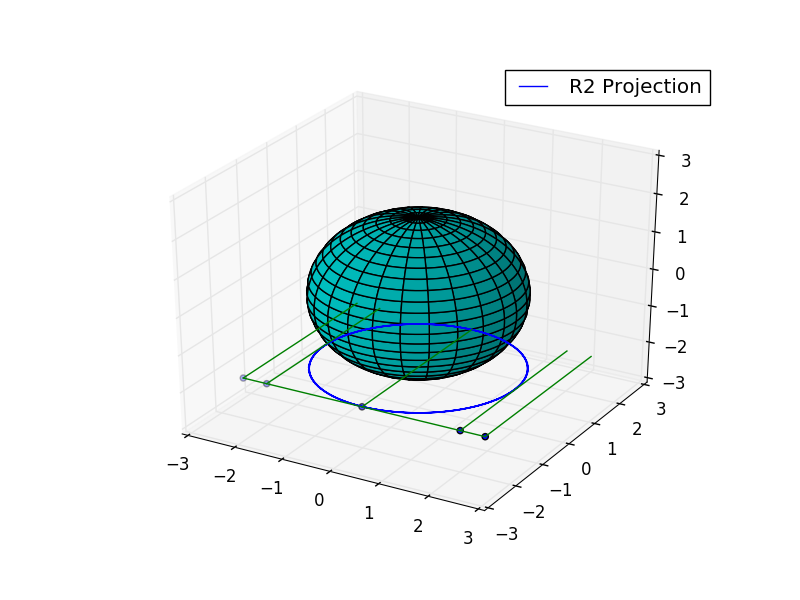
\includegraphics[width=1\textwidth]{sphereR3.png}
\end{figure}
\end{frame}

\begin{frame}{Example 1: the sphere}{Projection}
    \begin{itemize}
   		\item Input: $A = \{\:Poly(x^{2} + y^{2} + z^{2}-4)\:\}$
        \newline
        \item Output:
        \begin{itemize}
        	\item $A = \{\:Poly(x^{2} + y^{2} + z^{2}-4)\:\}$
        	\item $PROJ(A) = \{\:Poly(x^{2} + y^{2} - 4)\:\}$
    		\item $PROJ^{2}(A) = \{\:Poly(x + 2), \: \: \: Poly(x - 2)\:\}$
        \end{itemize}
    \end{itemize}
\end{frame}

%\subsection{Extension}
\begin{frame}{Example 1: the sphere}{Extension}
\begin{figure}
\includegraphics[width=1\textwidth]{SphereExtension.png}
\end{figure}
\end{frame}


\section{Example 2: a paraboloid and a cylinder}
\begin{frame}{Example 2: a paraboloid and a cylinder}
\begin{figure}
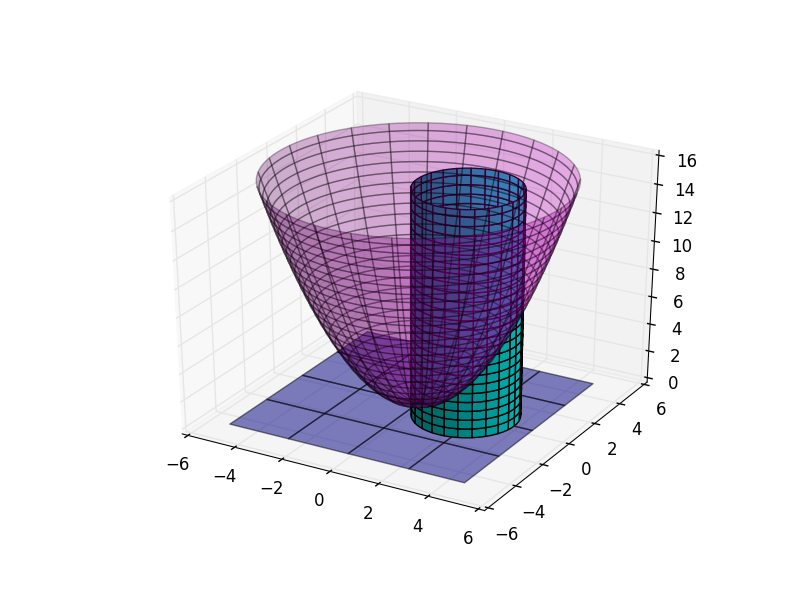
\includegraphics[width=1\textwidth]{paraboloideconcilindro.png}
\end{figure}
\end{frame}


\section{Falls and comebacks}
\begin{frame}{Falls and comebacks}{Projection}
    \begin{itemize}
        \item Different definitions of the same function
        \item Special cases
        \item Iterating the projection function
        \item Different process described in different references
    \end{itemize}
\end{frame}


\begin{frame}{Falls and comebacks}{Lifting}
    \begin{itemize}
        \item The issue with eval function.
        \item Compute with algebraic numbers
        \item Learn algebra.
        \item Making tests.
    \end{itemize}
\end{frame}

\begin{frame}{Computing with algebraic numbers}{Lifting}
    \begin{itemize}
        \item The issue with eval function.
        \begin{itemize}
        \item Symbolic method to find roots of polynomials: \emph{only for rational coefficients}
        \end{itemize}
        \item Computing with algebraic numbers
        \begin{itemize}
        \item We represent an algebraic number with a polynomial and and interval
        \item Operations on algebraic numbers become operations with polynomials        
        \end{itemize}
		\begin{exampleblock}{Algorithm}
        IN: Polynomial with \emph{algebraic} coefficients with roots $\{\alpha_i\}$
        
        OUT: A polynomial with \emph{rational} coefficients with $\{\alpha_i\}$ among its roots
        \end{exampleblock}
    \end{itemize}
\end{frame}


\section{Left to do}
\begin{frame}{Left to do}
    \begin{itemize}
        \item Optimization of the algorithm
        \item Refine the code to handle every case correctly
        \item Adapt code format to Python and Sympy standards
        \item Implement the quantifier elimination using the cad.
    \end{itemize}
\end{frame}


\section{Behind the scenes}
\begin{frame}{Behind the scenes}
    \begin{block}{Theorem}
		Let $\mathcal{D}$ be a domain and 0 $\leq$ j $\leq$ min(p, q) if p $\neq$ q (resp. 0 $\leq$ j $\leq$ p - 1 if p $=$ q).  Then deg(gcd(P, Q)) $\geq$ j if and only if
        $$sRes_0(P, Q) = \cdots = sRes_{j-1}(P, Q) = 0$$
	\end{block}
\end{frame}


\section{QA}
\begin{frame}{QA}
    \centering
        Questions? 
    \begin{figure}
     
\includegraphics[width=0.5\textwidth]{holiday-octocat.png}
    \end{figure}
   \end{frame}


%\begin{frame}{Example}
    
%\end{frame}


\end{document}


